\documentclass[10pt,a4paper]{article}
\usepackage[margin=20mm]{geometry}
\usepackage{booktabs,amsmath,graphicx,microtype,xcolor,pgfplots}
\pgfplotsset{compat=1.18}
\usepackage[colorlinks=true,urlcolor=blue,linkcolor=blue]{hyperref}
\usepackage{enumitem}
\setlist{nosep,leftmargin=*}
\setlength{\parskip}{4pt}
\setlength{\parindent}{0pt}
\raggedbottom
\title{Frozen Cumulative-Demand Prefill Comparison}
\author{Session D: exploratory evidence record}
\date{9 October 2026}
\hypersetup{pdftitle={Frozen Cumulative-Demand Prefill Comparison},pdfauthor={Session D},pdfsubject={Negative exploratory result; not a submission-ready paper}}
\begin{document}
\maketitle
\vspace{-5mm}
\textbf{Decision: retain fixed1024 and close this mapping in the tested operating domain.}
This record preserves a completed negative comparison. It establishes neither a new
method contribution nor a general impossibility result. The overall research and
submission objective remains incomplete; the historical manuscript is unchanged.

\section*{Question and intervention}
Can a simple cumulative prefill-demand rule retain the generation benefit of small
chunks without paying a larger waiting cost? Earlier fixed512 comparisons motivated
this question: shorter generation spans did not translate into faster completion.
The present experiment tests one frozen rule, not a tuned family of revisions.

The only controlled action is the aggregate number of prefill tokens permitted in
one native scheduler step. Admission, request order, decoder progress, KV allocation,
recovery, model precision, and operators remain common. For the native-order prefix
of unfinished prompts that have already arrived, the rule computes
\[
 r(t)=\max_j\frac{\sum_{i\leq j}p_i^{\mathrm{remaining}}}{a_j+4-t}.
\]
It selects the smallest pure-prefill cap in $\{512,1024,2048\}$ whose predicted
processing rate meets $r(t)$. The same frozen mixed-step cost model, multiplied by
1.2, supplies the denominator. Expired deadlines or an infeasible/invalid prediction
select 2048 as a progress fallback; none of these fallbacks occurred in the two
measured demand runs. This is an adaptation of a classical arrived-work demand
principle\footnote{Yao, Demers, and Shenker, FOCS 1995, Sections 3--4:
\href{https://perso.ens-lyon.fr/loris.marchal/scheduling/Yao-FOCS95-Energy.pdf}{author-hosted paper}.},
not a new scheduling principle or a deadline guarantee. Underfilling,
changing decoder load, and future arrivals prevent transferring a fluid feasibility
argument to this system.

\section*{Deployment and measurement}
The runtime is in-process vLLM 0.26 with PyTorch 2.11 and CUDA 13, serving BF16
OLMoE-1B-7B-0924-Instruct on one RTX PRO 6000 Blackwell GPU. Normal memory allocation
uses a 0.9 device-memory target and 588,032 usable KV tokens. The engine permits
192 sequences, a 4,096-token model length, and a 4,096-token native step budget.
Prefix caching and asynchronous scheduling are disabled. No artificial small-KV
limit, preemption, or recovery intervention is used.

All arms receive the same 256 open-loop requests: 128 QMSum long prompts and
128 GSM8K short prompts, with 538,597 prompt tokens and 114,688 declared output
tokens. Arrivals end at approximately 31.87 seconds; observation continues through
drain, with a 180-second timeout. EOS is ignored for this fixed-output diagnostic.
Planned external arrivals define TTFT and completion latency, including submission
lag. Token timestamps are host observations after synchronous \texttt{engine.step()}
returns, not isolated GPU kernel times.

The frozen research contract requires TTFT $\leq4$ seconds, each request's maximum
successive-output gap $\leq100$ ms, and completion latency $\leq20$ seconds.
Joint goodput $U$ is the number meeting all three divided by the full elapsed
service time, including waiting and drain. These thresholds have no established
production justification. They were not changed after observing this comparison.

The order was fixed1024, demand, demand, fixed1024 after four warmups in a shared
compilation domain. Warmups exercised all three fixed caps at their actual limits.
No compilation or graph capture was recorded after measurement began. Each measured
arm completed all 256 requests, with no failure, rejection, timeout, unfinished
request, or preemption.

\section*{Complete-service results}
% Generated by prefill_demand/render_results.py; no floating wrapper.
% Requires booktabs. Width170mm; max-gap column is milliseconds.
\begingroup\small\setlength{\tabcolsep}{4pt}
\begin{tabular*}{170mm}{@{\extracolsep{\fill}}lrrrrrr@{}}
\toprule
Cell / policy & Qualified & $U$ (req/s) & Elapsed (s) & TTFT p95 (s) & Flow p95 (s) & Gap p95 (ms) \\
\midrule
00 / Fixed 1024 & 183/256 & 3.7100 & 49.326 & 2.033 & 23.042 & 57.928 \\
01 / Demand & 151/256 & 2.9722 & 50.804 & 3.348 & 24.932 & 56.311 \\
02 / Demand & 153/256 & 3.0138 & 50.767 & 3.362 & 24.889 & 62.508 \\
03 / Fixed 1024 & 183/256 & 3.7078 & 49.355 & 2.057 & 23.116 & 66.928 \\
\bottomrule
\end{tabular*}\par
\endgroup

\par
Pair 1 compares demand cell 01 with fixed cell 00; pair 2 compares demand cell 02
with fixed cell 03. These are two reverse-order repetitions of one already-seen
development trace, not independent workload confirmation. The figure and table
are generated directly from the retained analysis JSON files.

\begin{figure}[!ht]
\centering
% Generated from service_decomposition.json; requires tikz and pgfplots.
% No figure float. Pair1=F00/D01; Pair2=F03/D02. Changes are Demand minus Fixed.
% TTFT is the first-output interval, not isolated queue time. Full elapsed defines U.
% Mean finish-remainder changes (s): 0.000000000, 0.000000000
\begin{minipage}[t]{0.49\linewidth}
\centering
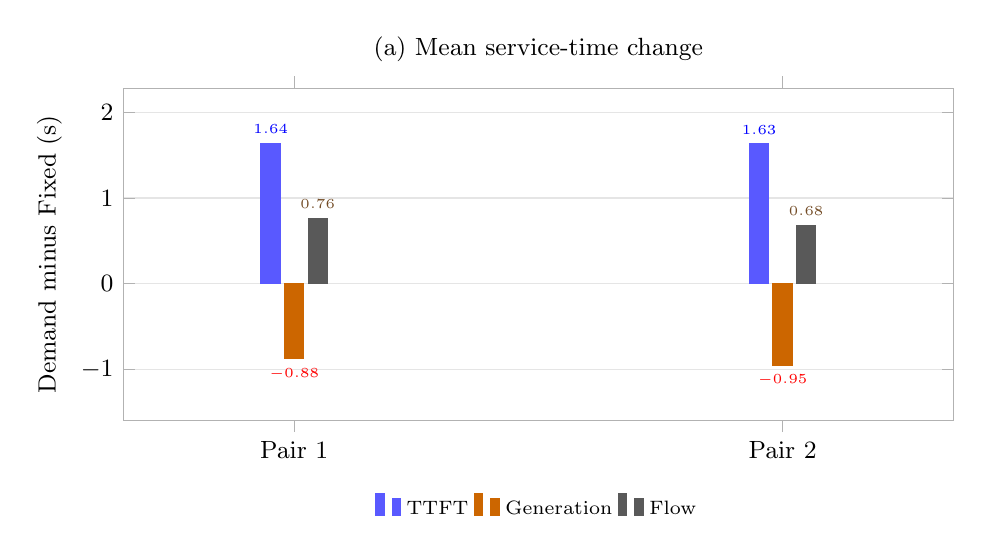
\begin{tikzpicture}
\begin{axis}[width=\linewidth,height=58mm,
font=\small,ybar=1.5pt,bar width=7pt,
symbolic x coords={Pair 1,Pair 2},xtick=data,
enlarge x limits=0.35,enlarge y limits=0.25,
ymajorgrids=true,grid style={gray!20},axis line style={gray!60},
tick style={gray!60},scaled y ticks=false,
title={(a) Mean service-time change},ylabel={Demand minus Fixed (s)},
nodes near coords,point meta=y,
every node near coord/.append style={font=\tiny,/pgf/number format/fixed,
/pgf/number format/precision=2},
legend style={at={(0.5,-0.2)},anchor=north,draw=none,font=\scriptsize},
legend columns=3]
\addplot+[fill=blue!65,draw=blue!65] coordinates {(Pair 1,1.636617490) (Pair 2,1.632100402)};
\addlegendentry{TTFT}
\addplot+[fill=orange!80!black,draw=orange!80!black] coordinates {(Pair 1,-0.877897588) (Pair 2,-0.951251844)};
\addlegendentry{Generation}
\addplot+[fill=black!65,draw=black!65] coordinates {(Pair 1,0.758719902) (Pair 2,0.680848557)};
\addlegendentry{Flow}
\end{axis}
\end{tikzpicture}
\end{minipage}
\hfill%
\begin{minipage}[t]{0.49\linewidth}
\centering
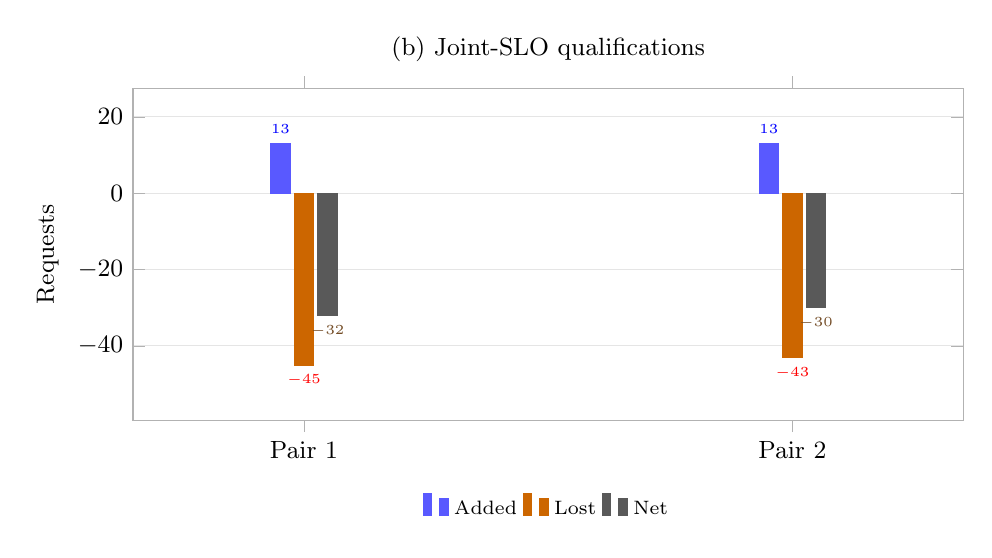
\begin{tikzpicture}
\begin{axis}[width=\linewidth,height=58mm,
font=\small,ybar=1.5pt,bar width=7pt,
symbolic x coords={Pair 1,Pair 2},xtick=data,
enlarge x limits=0.35,enlarge y limits=0.25,
ymajorgrids=true,grid style={gray!20},axis line style={gray!60},
tick style={gray!60},scaled y ticks=false,
title={(b) Joint-SLO qualifications},ylabel={Requests},
nodes near coords,point meta=y,
every node near coord/.append style={font=\tiny,/pgf/number format/fixed,
/pgf/number format/precision=0},
legend style={at={(0.5,-0.2)},anchor=north,draw=none,font=\scriptsize},
legend columns=3]
\addplot+[fill=blue!65,draw=blue!65] coordinates {(Pair 1,13.000000000) (Pair 2,13.000000000)};
\addlegendentry{Added}
\addplot+[fill=orange!80!black,draw=orange!80!black] coordinates {(Pair 1,-45.000000000) (Pair 2,-43.000000000)};
\addlegendentry{Lost}
\addplot+[fill=black!65,draw=black!65] coordinates {(Pair 1,-32.000000000) (Pair 2,-30.000000000)};
\addlegendentry{Net}
\end{axis}
\end{tikzpicture}
\end{minipage}

\caption{Demand minus contemporaneous fixed1024. Waiting increases exceed
generation-span reductions. Qualified additions are outweighed by losses in both
pairs. These are differences between full policy trajectories, not matched-state
causal effects. All 256 requests enter each pair's statistics.}
\end{figure}

Both demand runs improve qualification for the same 13 of the baseline's 73
completion-only failures. They introduce 45 and 43 new completion-only failures,
respectively. There are no new TTFT or maximum-gap violations: remaining inside the
TTFT threshold does not make the additional waiting harmless to completion.
For all 73 original failures, generation becomes shorter and TTFT becomes longer;
their mean completion latency nevertheless increases in both pairs.

Goodput decreases by 19.89\% and 18.72\%. Raw output throughput decreases by
2.91\% and 2.78\%, while full elapsed time increases by 1.479 and 1.412 seconds.
Thus the outcome is not a qualification gain masked by a longer denominator, nor
a gain obtained by shortening drain. Both the qualified-request numerator and
elapsed-time denominator move against demand. Per-request maximum-gap P95 improves
by 2.79\% and 6.60\%; this benefit is retained in the report rather than treated
as evidence of an overall win.

\section*{Execution evidence, interpretation, and limits}
The rule actually changes execution on 727 and 726 steps: 724 binding reductions
below 1024 in each run and 3/2 steps executing more than 1024 prefill tokens.
There are no zero-prefill steps with a backlog. Total measured controller time is
approximately 0.103 seconds per demand run versus 0.057 seconds for fixed1024;
all of it remains included in elapsed time. Peak KV occupancy is approximately
62\% for demand and 66\% for fixed1024, so this comparison is not a capacity-eviction
experiment.

The descriptive identity is completion latency = TTFT + first-to-last-output span
+ last-output-to-completion remainder. The last term is zero here. This identity
does not assign causal shares to overlapping GPU work. Equal prompt/output counts
also do not imply equal contents, routing, computation, or quality: 254 requests
have different final token sequences in each paired comparison. Natural EOS and
semantic task quality were not evaluated.

\clearpage
\section*{Decision and reproducibility}
The result rejects this frozen mapping for this operating domain and joint objective.
It does not refute the broader problem or establish fixed1024 as globally optimal.
Niyama already combines deadlines and estimated remaining service; Sarathi-Serve
and SLOWeave already address chunking and decode interference.\footnote{Primary sources:
\href{https://arxiv.org/html/2503.22562v1}{Niyama},
\href{https://arxiv.org/abs/2403.02310}{Sarathi-Serve},
\href{https://arxiv.org/html/2609.07883v1}{SLOWeave}.
See \texttt{NEIGHBORS.txt} for component boundaries.}
No full-system
superiority over these neighbors is claimed. Positive-only follow-ups such as
head-only or mean-work-matched controls are not launched to rescue this negative
result. Further investment requires a separately justified question and new evidence.

\textbf{Retained failure and commands.}
The preceding attempt, \texttt{demand53005\_01}, stopped at the disk-space guard
before model initialization: zero warmups and zero measured runs. Its records are
retained as a resource failure, not a negative method result.

From \path{D_prefill_budget_20261004/continuation_20261007}:
\begin{verbatim}
python3 -B prefill_demand/analyze_demand.py demand53005_02 \
  --design prefill_demand_resume/design.json
python3 -B prefill_demand/decompose_service.py demand53005_02
python3 -B prefill_demand/render_results.py
cd demand53005_02/presentation
pdflatex -interaction=nonstopmode -halt-on-error report.tex
\end{verbatim}
The sources are \path{demand53005_02/demand_results.json},
\path{demand53005_02/service_decomposition.json}, all eight retained raw files,
and the run log. The frozen design is \path{prefill_demand_resume/design.json};
the original rule is \path{prefill_demand/controller.py}. Code hashes and full
request migrations remain in the JSON and \path{RESULTS.md}. These commands
reproduce analysis and this record; they do not launch a new GPU experiment.
\end{document}
